%!TEX root = ../draft.tex

\begin{appendices}
% \adjustmtc 
\renewcommand{\appendixname}{ANHANG}
\renewcommand{\appendixtocname}{\appendixname} 
\addappheadtotoc 

% \begin{mtchideinmaintoc}[0]   %  [-1] Den folgenden Inhalt nicht im großen Inhaltsverzeichnis zeigen, [0] ab Chapter im großen Inhaltsverzeichnis anzeigen

\part*{Anhang}

\chapter{Fragebogen}
\label{anh:fragebogen}

\begin{figure}[!htb]
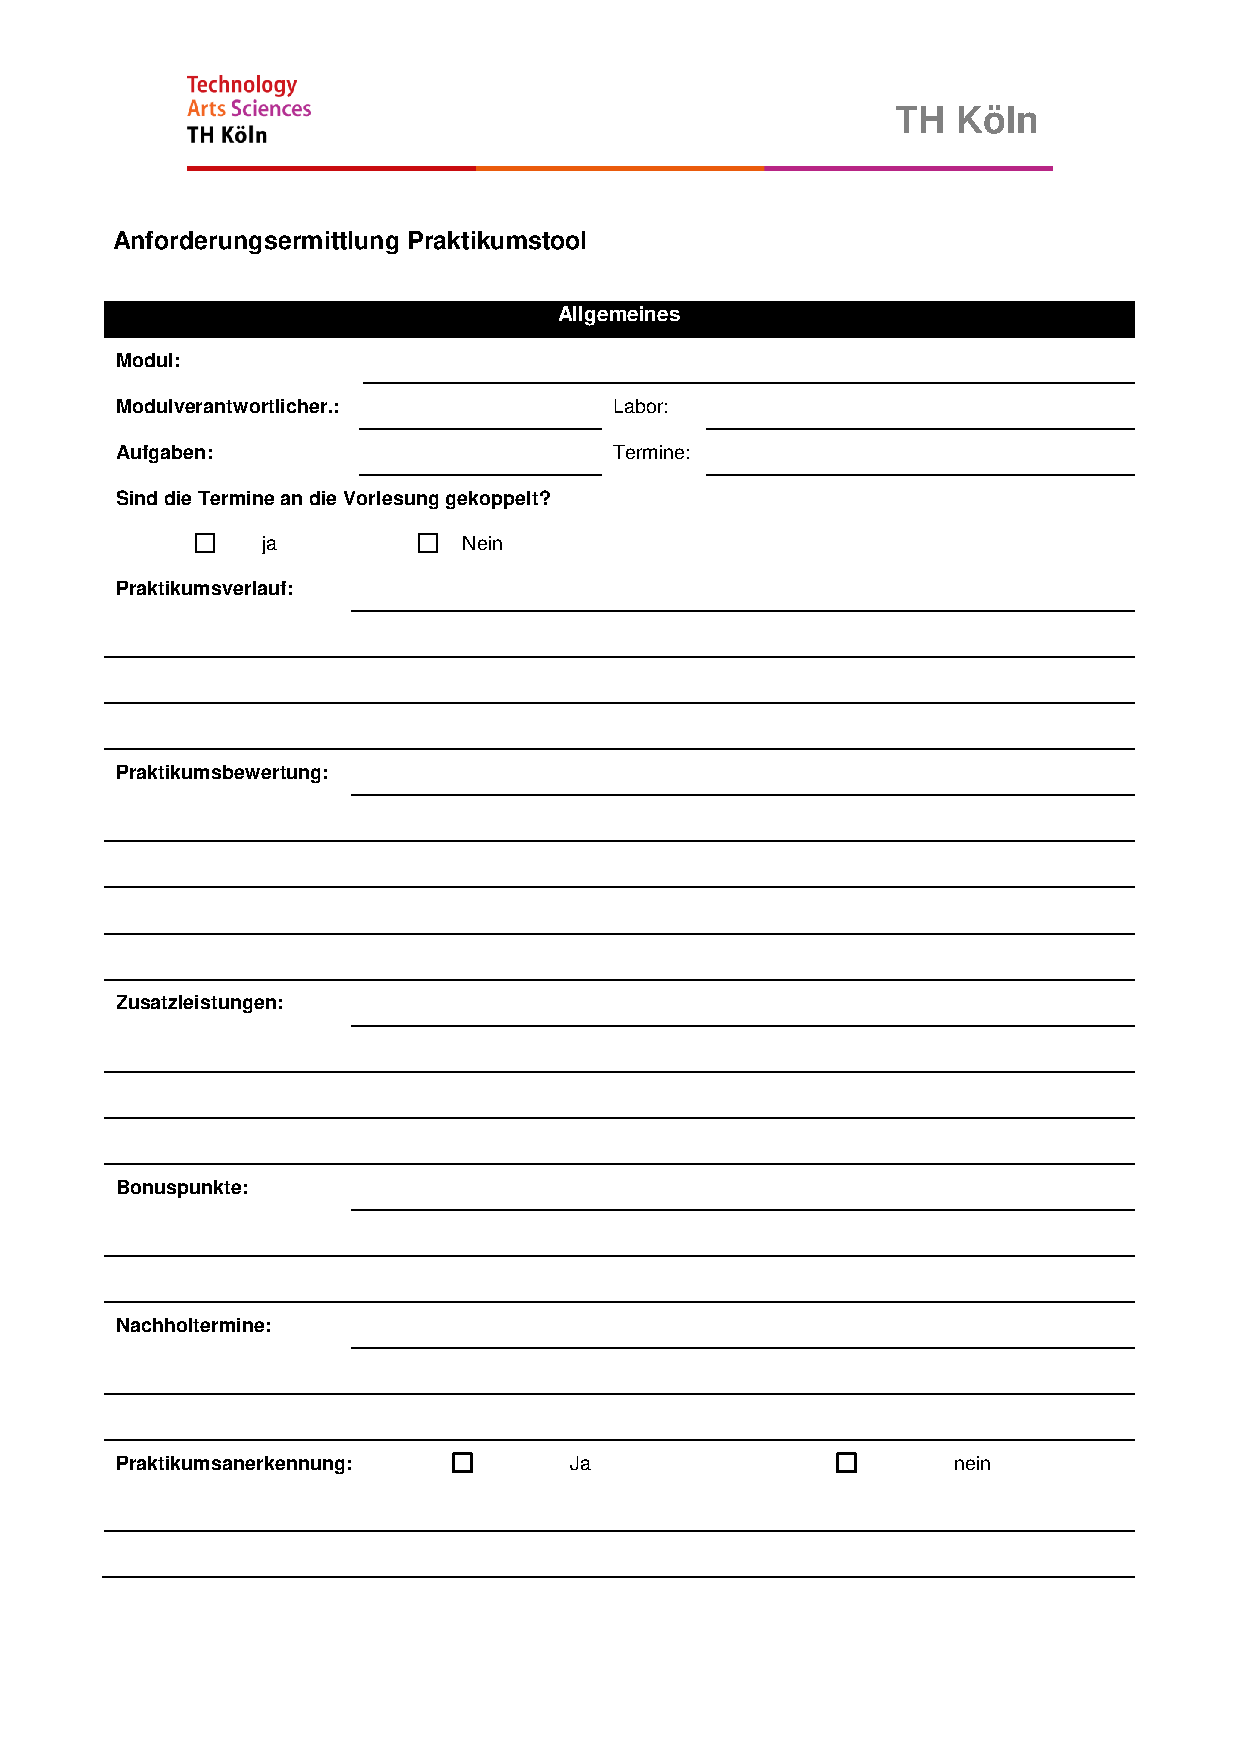
\includepdf[pages=1, width=.95\textwidth]{anhang/Fragebogen.pdf}
\end{figure}

\includepdf[pages=2, width=.95\textwidth]{anhang/Fragebogen.pdf}

\end{appendices}